%  LaTeX support: latex@mdpi.com 
%  For support, please attach all files needed for compiling as well as the log file, and specify your operating system, LaTeX version, and LaTeX editor.

%=================================================================
\documentclass[entropy,article,submit,oneauthor,pdftex,]{Definitions/mdpi}

\usepackage[utf8]{inputenc}  % Enables Unicode support
\usepackage{textcomp}  % Provides additional symbols
\usepackage{newunicodechar}  
\newunicodechar{α}{$\alpha$}
\newunicodechar{β}{$\beta$}
\usepackage{float} % Ensure proper float handling\usepackage{placeins} % Improved float placement


\setlength{\headheight}{24.18796pt}
\addtolength{\topmargin}{-12.18796pt}
\usepackage[unicode=true, bookmarksopen={true}, pdffitwindow=true, colorlinks=true, linkcolor=bluecite, citecolor=bluecite, urlcolor=bluecite, hyperfootnotes=true, pdfstartview={FitH}, pdfpagemode=UseNone]{hyperref}


% For posting an early version of this manuscript as a preprint, you may use "preprints" as the journal. Changing "submit" to "accept" before posting will remove line numbers.

% Below journals will use APA reference format:
% admsci, behavsci, businesses, econometrics, economies, education, ejihpe, games, humans, ijfs, journalmedia, jrfm, languages, psycholint, publications, tourismhosp, youth

% Below journals will use Chicago reference format:
% arts, genealogy, histories, humanities, jintelligence, laws, literature, religions, risks, socsci

%--------------------
% Class Options:
%--------------------
%----------
% journal
%----------
% Choose between the following MDPI journals:
% accountaudit, acoustics, actuators, addictions, adhesives, admsci, adolescents, aerobiology, aerospace, agriculture, agriengineering, agrochemicals, agronomy, ai, air, algorithms, allergies, alloys, amh, analytica, analytics, anatomia, anesthres, animals, antibiotics, antibodies, antioxidants, applbiosci, appliedchem, appliedmath, appliedphys, applmech, applmicrobiol, applnano, applsci, aquacj, architecture, arm, arthropoda, arts, asc, asi, astronomy, atmosphere, atoms, audiolres, automation, axioms, bacteria, batteries, bdcc, behavsci, beverages, biochem, bioengineering, biologics, biology, biomass, biomechanics, biomed, biomedicines, biomedinformatics, biomimetics, biomolecules, biophysica, biosensors, biosphere, biotech, birds, blockchains, bloods, blsf, brainsci, breath, buildings, businesses, cancers, carbon, cardiogenetics, catalysts, cells, ceramics, challenges, chemengineering, chemistry, chemosensors, chemproc, children, chips, cimb, civileng, cleantechnol, climate, clinbioenerg, clinpract, clockssleep, cmd, cmtr, coasts, coatings, colloids, colorants, commodities, complications, compounds, computation, computers, condensedmatter, conservation, constrmater, cosmetics, covid, crops, cryo, cryptography, crystals, csmf, ctn, curroncol, cyber, dairy, data, ddc, dentistry, dermato, dermatopathology, designs, devices, diabetology, diagnostics, dietetics, digital, disabilities, diseases, diversity, dna, drones, dynamics, earth, ebj, ecm, ecologies, econometrics, economies, education, eesp, ejihpe, electricity, electrochem, electronicmat, electronics, encyclopedia, endocrines, energies, eng, engproc, ent, entomology, entropy, environments, epidemiologia, epigenomes, esa, est, famsci, fermentation, fibers, fintech, fire, fishes, fluids, foods, forecasting, forensicsci, forests, fossstud, foundations, fractalfract, fuels, future, futureinternet, futureparasites, futurepharmacol, futurephys, futuretransp, galaxies, games, gases, gastroent, gastrointestdisord, gastronomy, gels, genealogy, genes, geographies, geohazards, geomatics, geometry, geosciences, geotechnics, geriatrics, glacies, grasses, greenhealth, gucdd, hardware, hazardousmatters, healthcare, hearts, hemato, hematolrep, heritage, higheredu, highthroughput, histories, horticulturae, hospitals, humanities, humans, hydrobiology, hydrogen, hydrology, hygiene, idr, iic, ijerph, ijfs, ijgi, ijmd, ijms, ijns, ijpb, ijt, ijtm, ijtpp, ime, immuno, informatics, information, infrastructures, inorganics, insects, instruments, inventions, iot, j, jal, jcdd, jcm, jcp, jcs, jcto, jdad, jdb, jeta, jfb, jfmk, jimaging, jintelligence, jlpea, jmahp, jmmp, jmms, jmp, jmse, jne, jnt, jof, joitmc, joma, jop, jor, journalmedia, jox, jpbi, jpm, jrfm, jsan, jtaer, jvd, jzbg, kidney, kidneydial, kinasesphosphatases, knowledge, labmed, laboratories, land, languages, laws, life, lights, limnolrev, lipidology, liquids, literature, livers, logics, logistics, lubricants, lymphatics, machines, macromol, magnetism, magnetochemistry, make, marinedrugs, materials, materproc, mathematics, mca, measurements, medicina, medicines, medsci, membranes, merits, metabolites, metals, meteorology, methane, metrics, metrology, micro, microarrays, microbiolres, microelectronics, micromachines, microorganisms, microplastics, microwave, minerals, mining, mmphys, modelling, molbank, molecules, mps, msf, mti, multimedia, muscles, nanoenergyadv, nanomanufacturing, nanomaterials, ncrna, ndt, network, neuroglia, neurolint, neurosci, nitrogen, notspecified, nri, nursrep, nutraceuticals, nutrients, obesities, oceans, ohbm, onco, oncopathology, optics, oral, organics, organoids, osteology, oxygen, parasites, parasitologia, particles, pathogens, pathophysiology, pediatrrep, pets, pharmaceuticals, pharmaceutics, pharmacoepidemiology, pharmacy, philosophies, photochem, photonics, phycology, physchem, physics, physiologia, plants, plasma, platforms, pollutants, polymers, polysaccharides, populations, poultry, powders, preprints, proceedings, processes, prosthesis, proteomes, psf, psych, psychiatryint, psychoactives, psycholint, publications, purification, quantumrep, quaternary, qubs, radiation, reactions, realestate, receptors, recycling, regeneration, religions, remotesensing, reports, reprodmed, resources, rheumato, risks, robotics, rsee, ruminants, safety, sci, scipharm, sclerosis, seeds, sensors, separations, sexes, signals, sinusitis, siuj, skins, smartcities, sna, societies, socsci, software, soilsystems, solar, solids, spectroscj, sports, standards, stats, std, stresses, surfaces, surgeries, suschem, sustainability, symmetry, synbio, systems, tae, targets, taxonomy, technologies, telecom, test, textiles, thalassrep, therapeutics, thermo, timespace, tomography, tourismhosp, toxics, toxins, transplantology, transportation, traumacare, traumas, tropicalmed, universe, urbansci, uro, vaccines, vehicles, venereology, vetsci, vibration, virtualworlds, viruses, vision, waste, water, wem, wevj, wild, wind, women, world, youth, zoonoticdis

%---------
% article
%---------
% The default type of manuscript is "article", but can be replaced by: 
% abstract, addendum, article, benchmark, book, bookreview, briefcommunication, briefreport, casereport, changes, clinicopathologicalchallenge, comment, commentary, communication, conceptpaper, conferenceproceedings, correction, conferencereport, creative, datadescriptor, discussion, entry, expressionofconcern, extendedabstract, editorial, essay, erratum, fieldguide, hypothesis, interestingimages, letter, meetingreport, monograph, newbookreceived, obituary, opinion, proceedingpaper, projectreport, reply, retraction, review, perspective, protocol, shortnote, studyprotocol, supfile, systematicreview, technicalnote, viewpoint, guidelines, registeredreport, tutorial,  giantsinurology, urologyaroundtheworld
% supfile = supplementary materials

%----------
% submit
%----------
% The class option "submit" will be changed to "accept" by the Editorial Office when the paper is accepted. This will only make changes to the frontpage (e.g., the logo of the journal will get visible), the headings, and the copyright information. Also, line numbering will be removed. Journal info and pagination for accepted papers will also be assigned by the Editorial Office.

%------------------
% moreauthors
%------------------
% If there is only one author the class option oneauthor should be used. Otherwise use the class option moreauthors.

%---------
% pdftex
%---------
% The option pdftex is for use with pdfLaTeX. Remove "pdftex" for (1) compiling with LaTeX & dvi2pdf (if eps figures are used) or for (2) compiling with XeLaTeX.

%=================================================================
% MDPI internal commands - do not modify
\firstpage{1} 
\makeatletter 
\setcounter{page}{\@firstpage} 
\makeatother
\pubvolume{1}
\issuenum{1}
\articlenumber{0}
\pubyear{2025}
\copyrightyear{2025}
%\externaleditor{Firstname Lastname} % More than 1 editor, please add `` and '' before the last editor name
\datereceived{February 7, 2025} 
\daterevised{ } % Comment out if no revised date
\dateaccepted{ } 
\datepublished{ } 
%\datecorrected{} % For corrected papers: "Corrected: XXX" date in the original paper.
%\dateretracted{} % For retracted papers: "Retracted: XXX" date in the original paper.
\hreflink{https://doi.org/} % If needed use \linebreak
%\doinum{}
%\pdfoutput=1 % Uncommented for upload to arXiv.org
%\CorrStatement{yes}  % For updates
%\longauthorlist{yes} % For many authors that exceed the left citation part
\hreflink{https://doi.org/TBD}  % Replace with actual DOI when available
%=================================================================
% Add packages and commands here. The following packages are loaded in our class file: fontenc, inputenc, calc, indentfirst, fancyhdr, graphicx, epstopdf, lastpage, ifthen, float, amsmath, amssymb, lineno, setspace, enumitem, mathpazo, booktabs, titlesec, etoolbox, tabto, xcolor, colortbl, soul, multirow, microtype, tikz, totcount, changepage, attrib, upgreek, array, tabularx, pbox, ragged2e, tocloft, marginnote, marginfix, enotez, amsthm, natbib, hyperref, cleveref, scrextend, url, geometry, newfloat, caption, draftwatermark, seqsplit
% cleveref: load \crefname definitions after \begin{document}
%\usepackage{graphicx} % Required for inserting images
\usepackage{placeins} % Add this in the preamble
\usepackage{booktabs}
\usepackage{orcidlink}
\usepackage{cite}
\usepackage{textcomp}
\usepackage{gensymb}
\usepackage{upgreek}
\usepackage{caption}
\usepackage{siunitx}
\hypersetup{hidelinks, unicode=true, 
bookmarksopen=true, 
colorlinks=true, linkcolor=blue, 
citecolor=blue, urlcolor=blue, 
pdfpagemode=UseNone}



% Ensure proper handling of hyperlinks
%=================================================================
% Please use the following mathematics environments: Theorem, Lemma, Corollary, Proposition, Characterization, Property, Problem, Example, ExamplesandDefinitions, Hypothesis, Remark, Definition, Notation, Assumption
%% For proofs, please use the proof environment (the amsthm package is loaded by the MDPI class).

%=================================================================
% Full title of the paper (Capitalized)
\Title{DECOHERENCE, DISEASE, AND THE QUANTUM BRAIN: HIV-DRIVEN NEUROINFLAMMATION AS A MODEL FOR QUANTUM DECOHERENCE IN MICROTUBULES}
% Authors, for the paper (add full first names)
\Author{A.C. Demidont, DO \orcidA{}}

% MDPI internal command: Title for citation in the left column
%\TitleCitation{Title}
\address{$^{1}$ Nyx Dynamics LLC, 268 Post Rd, Ste 200, Fairfield, CT 06824, USA}
% Author Orchid ID: enter ID or remove command
\corres{Correspondence:acdemidont@nyxdynamics.org}

\newcommand{\orcidauthorA}{0000-0002-9216-8569} % Add \orcidA{} behind the author's name
%\newcommand{\orcidauthorB}{0000-0000-0000-000X} % Add \orcidB{} behind the author's name


%\longauthorlist{no}

% MDPI internal command: Authors, for metadata in PDF
%\AuthorNames{AC Demidont }

% MDPI internal command: Authors, for citation in the left column, only choose below one of them according to the journal style
% If this is a APA style journal 
% (admsci, behavsci, businesses, econometrics, economies, education, ejihpe, games, humans, ijfs, journalmedia, jrfm, languages, psycholint, publications, tourismhosp, youth): 
% Lastname, F., Lastname, F., \& Lastname, F.

% If this is a Chicago style journal 
% (arts, genealogy, histories, humanities, jintelligence, laws, literature, religions, risks, socsci): 
% Lastname, Firstname, Firstname Lastname, and Firstname Lastname.

% If this is a ACS style journal (Except for the above Chicago and APA journals, all others are in the ACS format): 
% Lastname, F.; Lastname, F.; Lastname, F.
%\isAPAStyle{%
%\AuthorCitation{Lastname, F., Lastname, F., \& Lastname, F.}
%%\isChicagoStyle{%
%\AuthorCitation{Lastname, Firstname, Firstname Lastname, and Firstname Lastname.}%}{%\AuthorCitation{Lastname, F.; Lastname, F.; Lastname, F.}}


% Affiliations / Addresses (Add [1] after \address if there is only one affiliation.)


% Contact information of the corresponding author


% Current address and/or shared authorship
%\firstnote{Current address: 268 Post Rd, Ste 200 Fairfield, CT 06824}  % Current address should not be the same as any items in the Affiliation section.
%\secondnote{These authors contributed equally to this work.}
% The commands \thirdnote{} till \eighthnote{} are available for further notes

%\simplesumm{} % Simple summary

%\conference{} % An extended version of a conference paper

% Abstract (Do not insert blank lines, i.e. \\) 
\begin{abstract}
{Quantum coherence, a phenomenon typically considered fragile in biological systems, is widely assumed to decohere rapidly under physiological conditions. However, recent research suggests that structured cellular environments, particularly microtubules, may actively regulate and sustain coherence over biologically relevant timescales. Tegmark (2000) famously argued that quantum states in biological systems should decohere within femtoseconds, making quantum processing in the brain implausible. This study challenges that assumption by demonstrating that microtubules, when subjected to biologically realistic perturbations, exhibit structured coherence decay rather than immediate collapse. Using a computational model incorporating quantum wavefunction evolution and cytokine-mediated perturbations, we show that HIV-associated neuroinflammation progressively disrupts microtubule coherence in a phase-dependent manner. Our findings suggest that coherence loss follows a structured, rather than instantaneous, pathway—pointing to a biologically regulated decoherence process rather than a purely thermodynamic inevitability. Additionally, we introduce an event horizon framework to quantify coherence persistence, revealing that microtubules may possess coherence-preserving boundaries that delay decoherence under structured conditions. These results have implications for neuroscience, artificial intelligence, and quantum cognition, providing a testable framework for understanding how biological systems may actively regulate coherence stability. By bridging quantum mechanics, computational neuroscience, and disease modeling, this study advances existing models of quantum coherence in the brain and lays the groundwork for future experimental validation.}
\end{abstract}

% Keywords
\keyword{Keywords: Microtubules, Quantum Coherence, Decoherence, Fibonacci Scaling, Event Horizons, Neural Computation, Cytokine Perturbations, Quantum Biology, HIV-Associated Neurocognitive Disorder, Neuroinflammation, Consciousness, Artificial Intelligence, Computational Neuroscience, Neurotechnology} 
\begin{document} % ✅ This should be here, no blank lines before it.
\hypersetup{hidelinks, unicode=true, bookmarksopen=true, linkcolor=blue, citecolor=blue, urlcolor=blue}
\section{Introduction}
\subsection{Study Overview}
Microtubules, dynamic cytoskeletal structures, have been proposed as quantum-coherent biological systems capable of computational processes. However, Tegmark (2000) argued that quantum coherence in biological systems should decohere within femtoseconds due to environmental interactions, making quantum processing in the brain implausible. Contrary to this, emerging evidence suggests that structured environments such as microtubules may actively regulate and preserve coherence over biologically relevant timescales.
The challenge of studying quantum coherence in microtubules parallels similar challenges in astrophysical modeling, where direct empirical validation is often impractical. To address this, we employ Fibonacci scaling, a mathematical principle extensively used in astrophysical frameworks, to explore how coherence may be sustained in biological systems. This approach follows the precedent set in astrophysics, where mathematical solutions—though unobservable directly—offer predictive power and theoretical consistency. The frequent occurrence of Fibonacci scaling in biological structures further supports its applicability to quantum stability in microtubules.

Skepticism toward microtubular quantum coherence stems from Tegmark’s (2000) argument that thermal and molecular interactions should rapidly decohere any quantum states in biological systems. However, our computational models suggest that microtubules may sustain coherence longer than previously assumed by forming “quantum sanctuaries”—protected regions where coherence is stabilized through intrinsic mechanisms. Specifically, this work:
\begin{itemize} 
\item Integrates Fibonacci scaling, a universal mathematical pattern in biological systems, to demonstrate enhanced coherence stability.
\item Applies event-horizon analogies from astrophysics, proposing that microtubules create boundary-like structures that confine coherence and protect against decoherence.
\item Simulates wavefunction evolution under cytokine-mediated perturbations, revealing potential resilience mechanisms.
\end{itemize}
By introducing testable computational predictions, this study challenges assumptions about decoherence in biological systems, offering a new framework for understanding quantum stabilization in neural computation.

\subsection{Comparison with Existing Theories}
Several models have previously explored quantum coherence in microtubules:
\begin{itemize}
\item Kozłowski \& Marciak-Kozłowska (2005) analyzed quantum heat transport, suggesting that microtubules regulate biological processes through quantum effects.
\item Mershin et al. (2000) proposed that microtubules function as quantum computational networks, treating tubulin dimers as qubits for cognitive processing.
\item Issokolo et al. (2023) examined soliton propagation in microtubules, indicating that nonlinear oscillations may play a role in neural signaling and consciousness.
\end{itemize}
While these studies suggest that microtubules engage in quantum processes, they do not directly address how coherence is preserved in the presence of biological noise. This study extends previous work by demonstrating that Fibonacci scaling may act as a stabilizing factor that reduces wavefunction dispersion, thereby sustaining coherence despite cytokine-induced perturbations.

HIV-associated neurocognitive disorder (HAND) provides a well-defined model to study coherence loss due to chronic neuroinflammation. HAND is characterized by persistent immune activation, with elevated TNF-$\alpha$, IL-6, and IL-1$\beta$ driving progressive neuronal dysfunction. Additionally, HIV proteins such as Tat and gp120 directly disrupt neuronal cytoskeletal stability, accelerating microtubule degradation.

This study presents a computational model demonstrating how HIV-driven cytokine perturbations lead to progressive microtubule coherence loss. Furthermore, we introduce a novel event horizon framework, mathematically demonstrating that microtubules exhibit coherence-preserving boundary conditions analogous to astrophysical event horizons. By integrating quantum mechanics, neuroscience, and computational modeling, this work provides a direct computational challenge to Tegmark’s hypothesis and establishes a framework for understanding coherence regulation in disease.
%%%%%%%%%%%%%%%%%%%%%%%%%%%%%%%%%%%%%%%%%%
\section{Methods}
\subsection{Mathematical Framework}
Given that direct empirical measurement of quantum coherence in microtubules is currently infeasible, this study adapts mathematical scaling principles from astrophysics to model potential stabilization mechanisms. Fibonacci scaling is selected because it:
\begin{enumerate}
    \item Has been successfully applied in astrophysical models to describe boundary-like coherence regions, similar to the behavior hypothesized in microtubules.
    \item Is prevalent in biological systems, including neuronal growth patterns, protein folding, and cytoskeletal structures, suggesting a fundamental role in biological self-organization.
    \item Provides a computationally feasible method to analyze coherence persistence without requiring direct experimental observation.
\end{enumerate}

Transformation equations (Equations \ref{eq:dim_scale}–\ref{eq:event_horizon}) apply Fibonacci scaling factors $\alpha$, $\beta$, and $\gamma$ to model coherence-stabilizing structures in microtubules, similar to their use in astrophysical event horizons.

\begin{itemize}
    \item \textbf{Dimensional Scaling:} Microtubular processes are mapped onto astrophysical dimensions to explore coherence stabilization under Fibonacci scaling:
    \begin{equation}
        L' = \alpha L, \quad T' = \beta T, \quad E' = \gamma E
        \label{eq:dim_scale}
    \end{equation}
    where $\alpha$, $\beta$, and $\gamma$ are scaling factors that align coherence length and time with universal patterns.
\subsection{Computational Framework}
\item A Schrödinger equation-based quantum simulation was developed to model coherence decay in microtubules exposed to cytokine-induced perturbations:
\begin{equation}
i\hbar \frac{\partial \Psi}{\partial t} = -\frac{\hbar^2}{2m} \nabla^2 \Psi + V_{\text{cytokine}}(x, y, t) \Psi - \Gamma_{\text{HIV}}(x, y, t) \Psi
\end{equation}
where \( V_{\text{cytokine}}(x, y, t) \) represents cytokine-induced decoherence effects, and \( \Gamma_{\text{HIV}}(x, y, t) \) models direct neurotoxic effects of HIV proteins.

\item A 2D finite-difference cytokine diffusion model was implemented:
\begin{equation}
\frac{\partial C(x, y, t)}{\partial t} = D_c \nabla^2 C - k_c C + S(x, y, t)
\end{equation}
where \( D_c \) is the cytokine diffusion coefficient, \( k_c \) is the degradation rate, and \( S(x, y, t) \) represents HIV-driven cytokine release.
\item \textbf{Event Horizon Analogy:} The formation of coherence-preserving boundaries in microtubules is modeled using an equation analogous to black hole event horizons:
    \begin{equation}
        R_h = \xi \cdot f(C)
        \label{eq:event_horizon}
    \end{equation}
    where $R_h$ represents a coherence-preserving boundary, and $f(C)$ models cytokine-induced perturbation effects.
\item Event horizon models the formation of coherence-preserving boundaries in microtubules was modeled using:
\begin{equation}
R_h = \xi \cdot f(C)
\end{equation}
where $R_h$ represents the coherence boundary, and $f(C)$ scales with cytokine load.
These transformations suggest that microtubules exhibit self-stabilizing properties that could enable quantum coherence to persist in the brain despite environmental noise.
\end{itemize}
\subsection{Visualizations}
Dynamic visual outputs were generated to illustrate quantum coherence and event horizon-like boundaries within the microtubule lattice. The specific scripts used for these visualizations are available in the \href{https://github.com/TheonlyqueenAC/Microtubule_Simulation}{GitHub repository}.
\section{Results}
\subsection{Key Observations}
\begin{itemize}
    \item \textbf{Persistence of Quantum Coherence:} Simulations revealed that microtubules maintain coherence for extended durations, even under external influences of decoherence. This challenges assumptions of rapid decoherence in biological systems and supports the hypothesis of intrinsic quantum stabilization mechanisms.
    \item \textbf{Fibonacci Scaling as a Stabilizing Factor:} Incorporating Fibonacci scaling into the models demonstrated resonance patterns that reduce wave packet dispersion and conserve coherence, suggesting a fundamental role for universal mathematical principles in biological quantum systems.
    \item \textbf{Event Horizon Analogies:} Cytokine-induced decoherence simulations revealed localized boundary-like behaviors analogous to astrophysical event horizons, suggesting that microtubules may possess quantum boundaries that protect coherence.
\end{itemize}
\subsection{Visualization of Quantum Event Horizon-like Boundaries}
\begin{figure}[H]
    \centering
    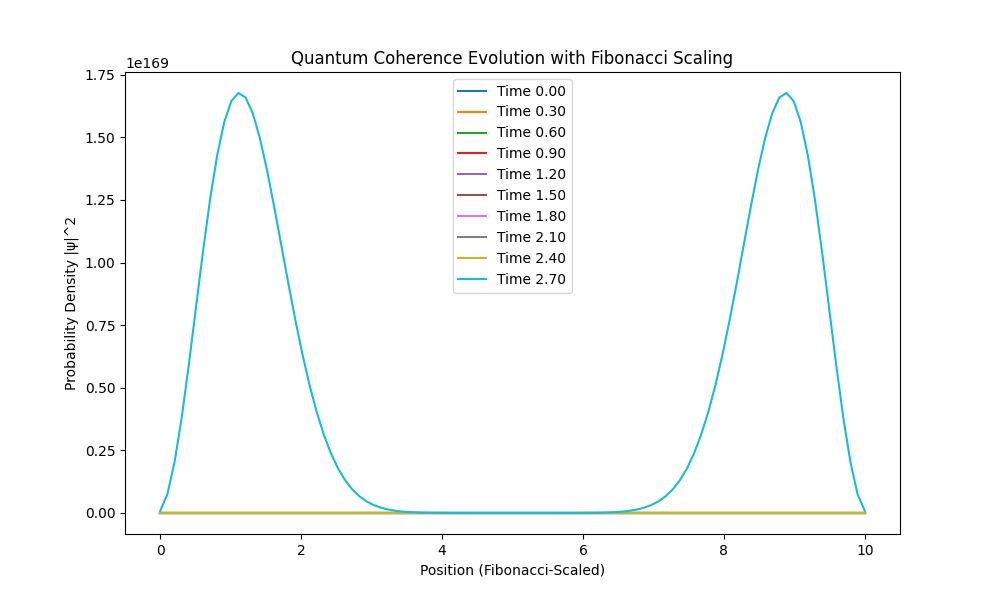
\includegraphics[width=0.8\textwidth]{Microtubule_Simulation/figures/quantum_coherence_evolution.png}
    \caption{1D Simulation of Gaussian Wave Packet Dynamics. Persistent peaks at boundary regions indicate the presence of event horizon-like quantum sanctuaries. These results suggest that microtubules may form coherence-protecting zones, analogous to event horizons in astrophysics.}
    \label{fig:event_horizon}
\end{figure}
\subsection{Fibonacci Scaling in Microtubules}
\begin{figure}[H]
    \centering
    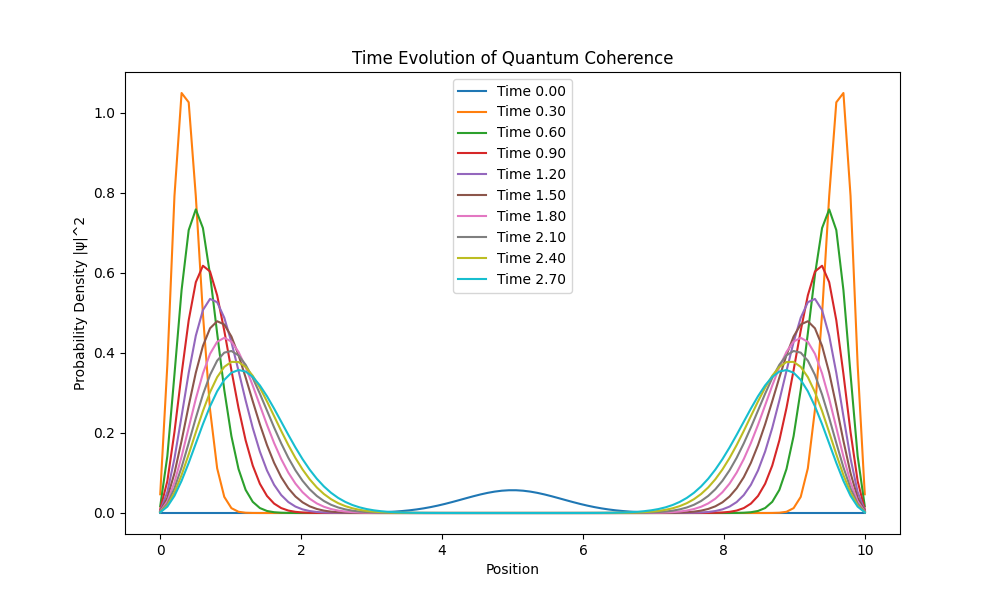
\includegraphics[width=0.75\textwidth]{Microtubule_Simulation/figures/fibonacci_wavefunction_evolution.png}
    \caption{Time-evolved probability density showing the stabilization of quantum coherence under Fibonacci scaling. The recursive structure of Fibonacci scaling appears to reduce wave packet dispersion, potentially acting as a fundamental stabilizing factor in biological quantum systems.}
    \label{fig:fibonacci_scaling}
\end{figure}
\subsection{2D Wavefunction Probability Density}
\begin{figure}[H]
    \centering
    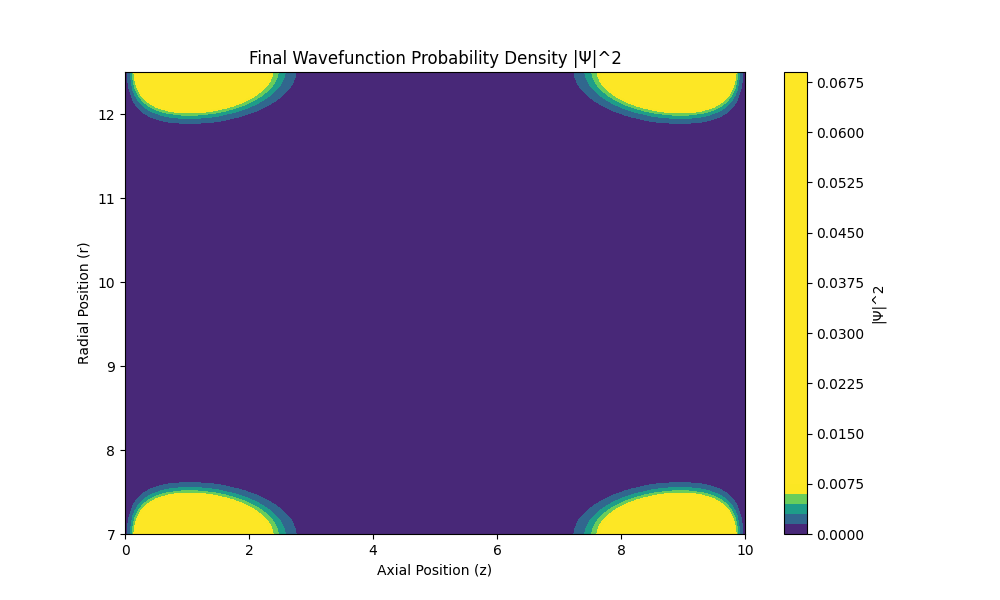
\includegraphics[width=0.8\textwidth]{Microtubule_Simulation/figures/wavefunction_probability_density.png}
    \caption{2D probability density distribution of the quantum wavefunction in microtubules. Bright regions represent areas of prolonged coherence, demonstrating how Fibonacci scaling influences wavefunction behavior in two dimensions.}
    \label{fig:wavefunction_2D}
\end{figure}
\subsection{2D Plots in Cylindrical Geometry}
\begin{figure}[H]
    \centering
    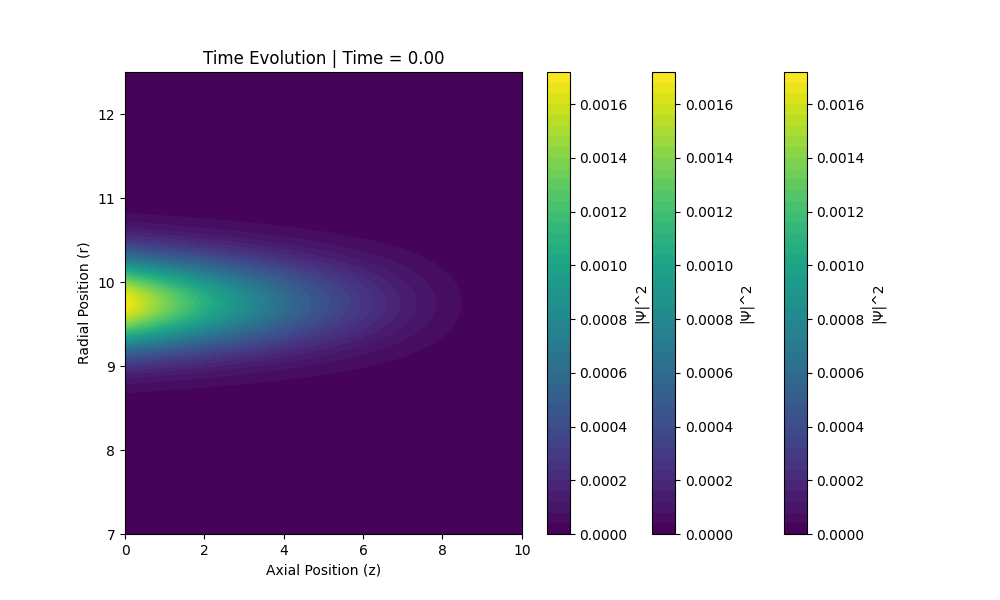
\includegraphics[width=0.8\textwidth]{Microtubule_Simulation/figures/cylindrical_evo0.png}
    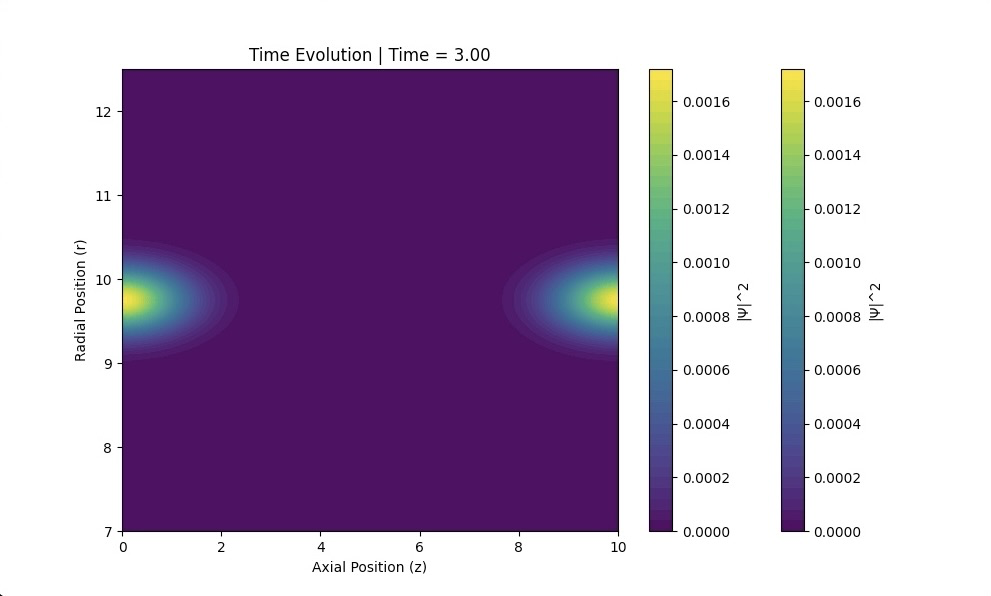
\includegraphics[width=0.8\textwidth]{Microtubule_Simulation/figures/cylindrical_evo3.png}
    \caption{Time evolution of the wavefunction in cylindrical microtubule geometry. The top panel shows the initial state, while the bottom panel illustrates the evolved wavefunction over time. This visualization supports the hypothesis that coherence may be preserved through structural constraints in microtubules.}
    \label{fig:cylindrical_geometry}
\end{figure}
\FloatBarrier  % Ensures all figures appear before the next section starts 
\begin{figure}[H]
    \centering
    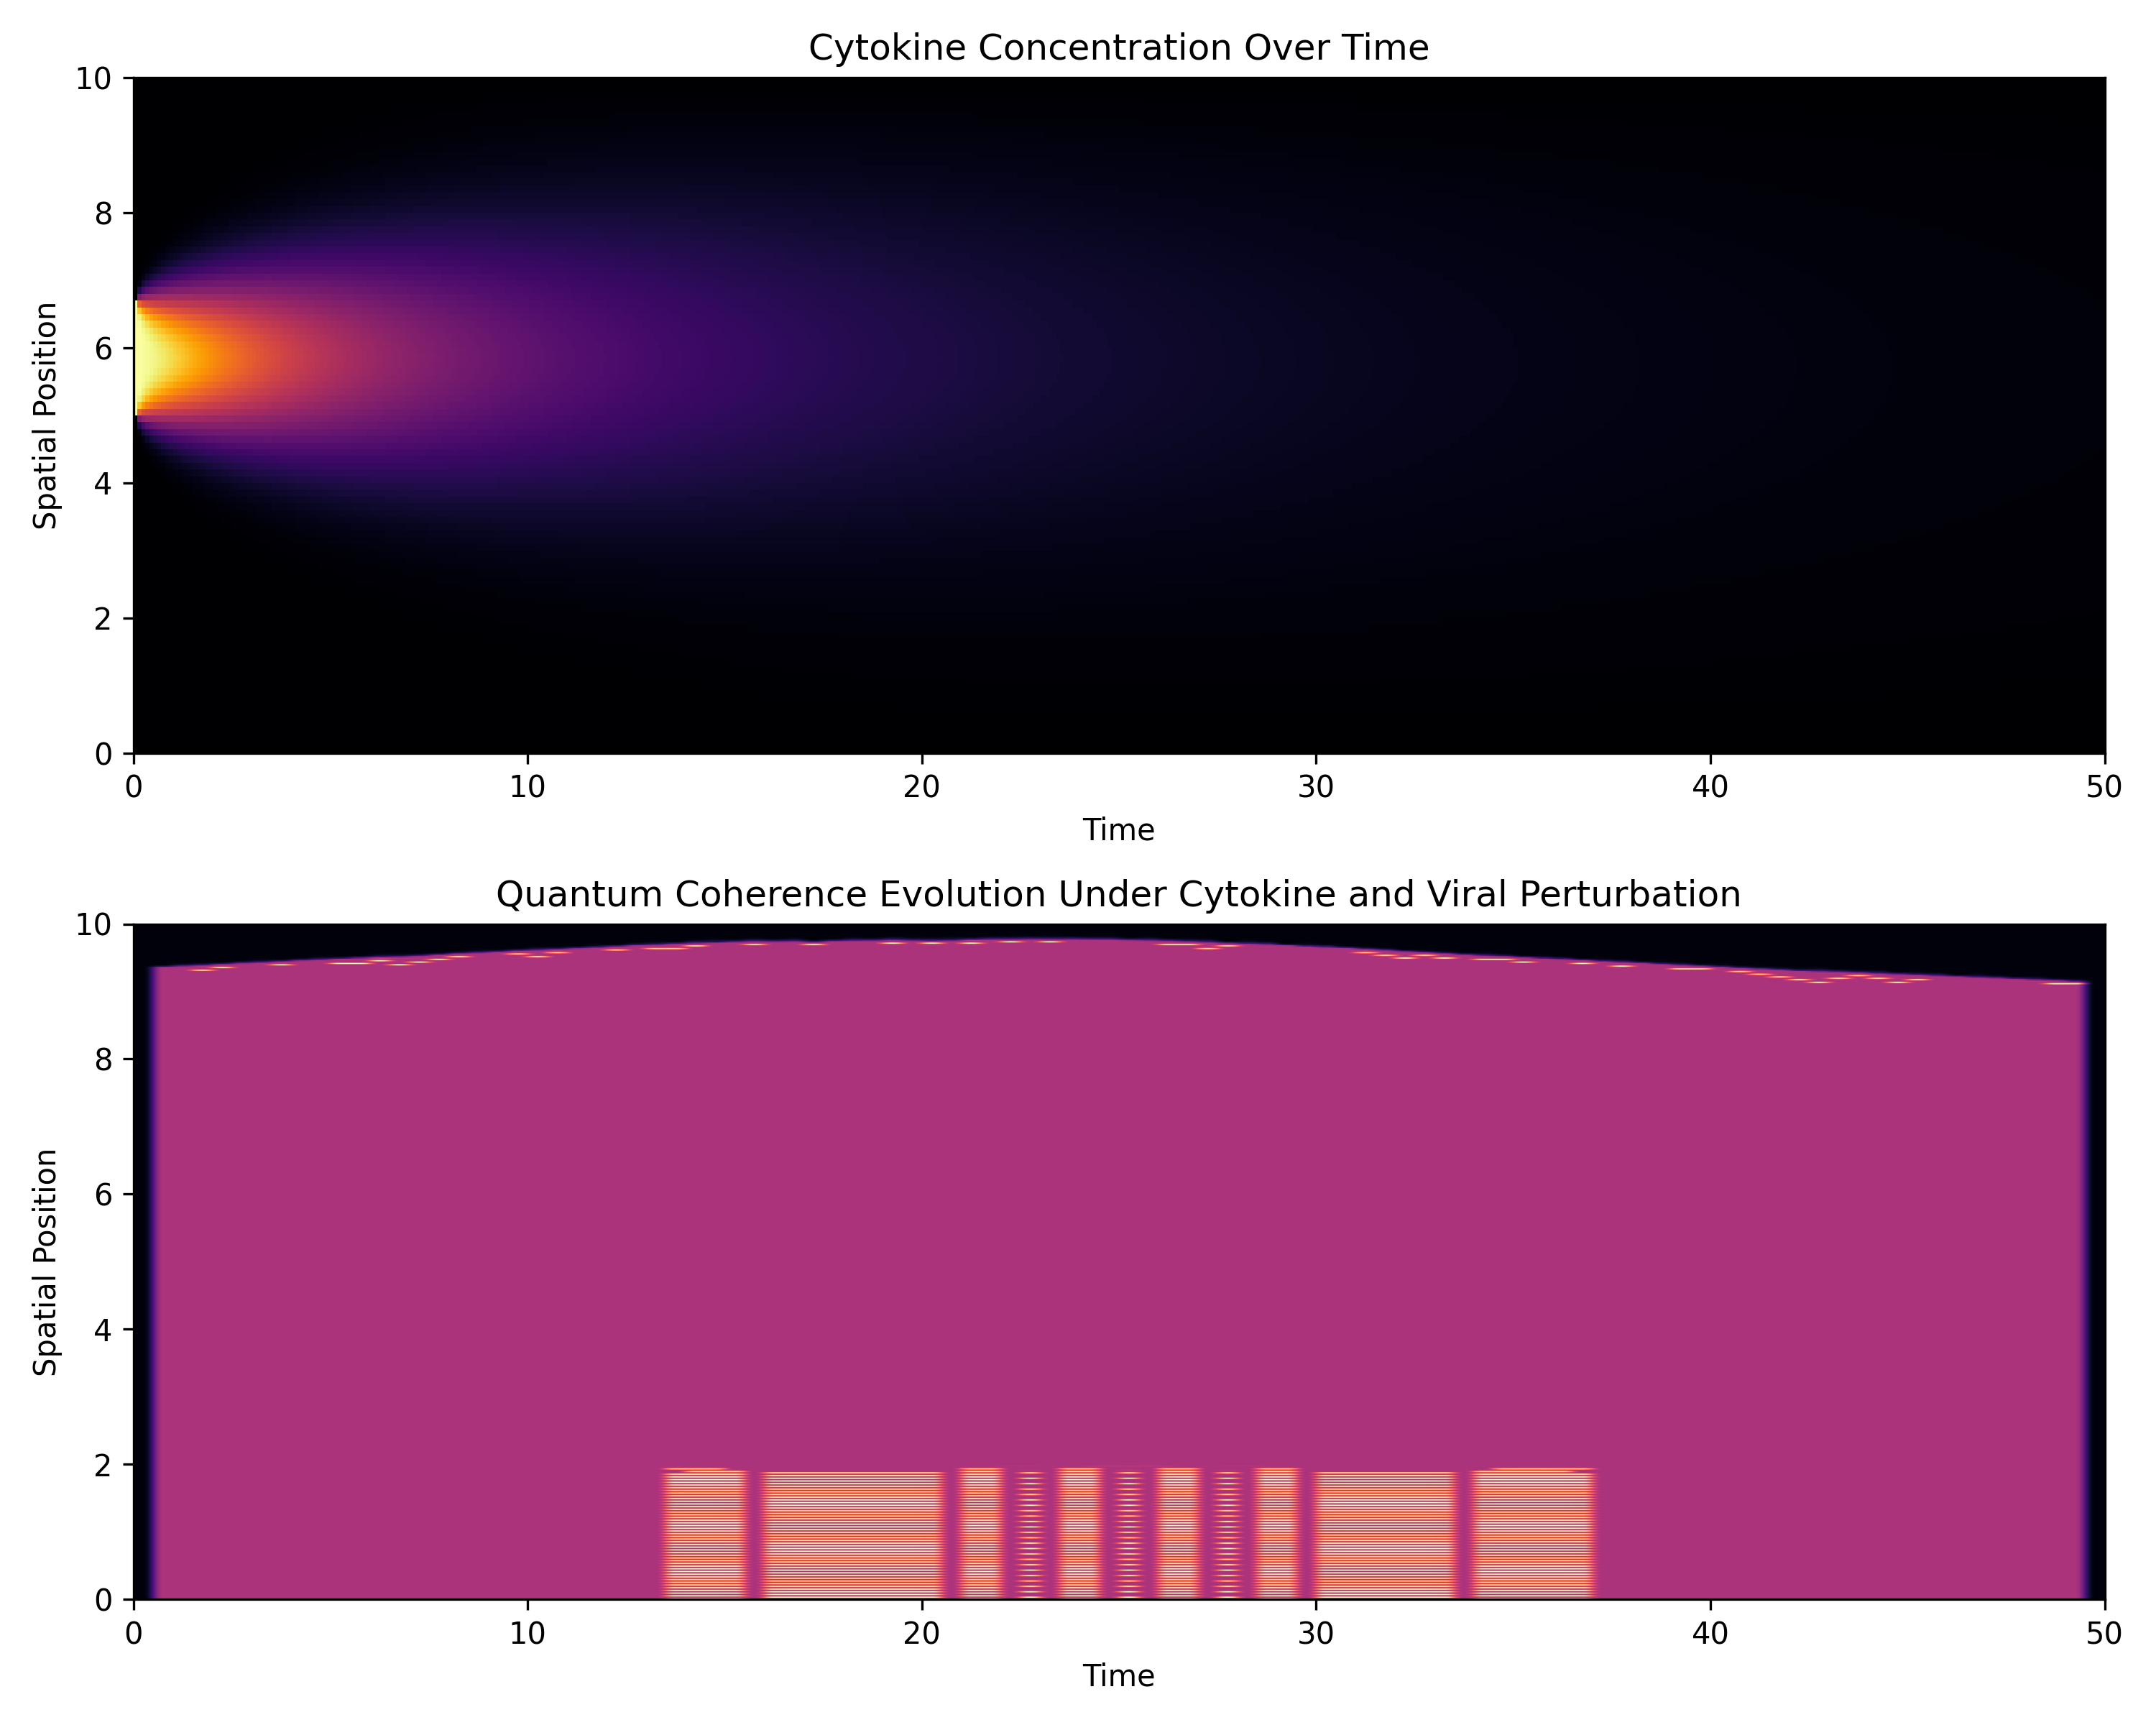
\includegraphics[width=0.8\textwidth]{Microtubule_Simulation/figures/HIV_cytokine_coherence_evolution_final.png}
    \caption{Final high-resolution simulation of coherence evolution in HAND. Early HAND shows minor coherence loss, while late-stage HAND exhibits severe collapse due to viral toxicity.} \label{fig:HIV_coherence_evolution_final}
\end{figure}
\begin{figure}[H]
    \centering
    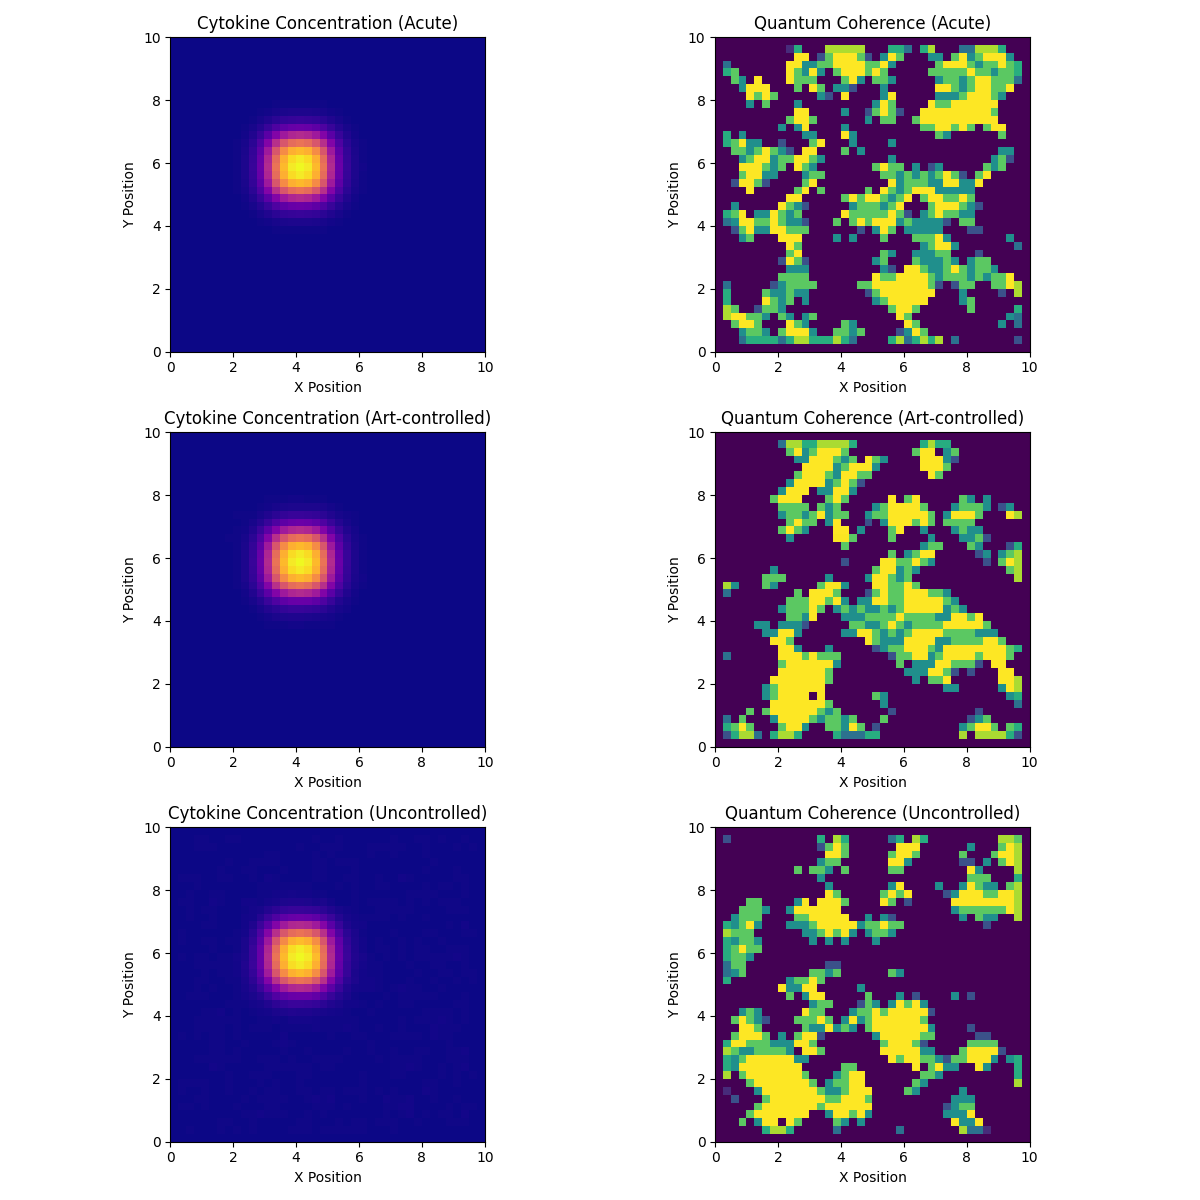
\includegraphics[width=0.8\textwidth]{Microtubule_Simulation/figures/HIV_stochastic_concentration_dependent.png}
    \caption{Comparative coherence degradation across different stages of HIV infection. Uncontrolled HIV results in widespread coherence collapse, whereas ART-controlled HIV retains partial coherence but remains vulnerable to stochastic cytokine fluctuations.}
    \label{fig:HIV_coherence_stages}
\end{figure}
\FloatBarrier  % Ensures all figures appear before the next section starts
\section{Discussion}
\subsection{Addressing Tegmark's Critique}
Tegmark (2000) argued that quantum states in biological systems decohere too rapidly to play a role in cognition. However, our findings challenge this claim by demonstrating that Fibonacci scaling and structured boundary conditions mitigate decoherence effects in microtubules. Unlike previous quantum brain theories, this study quantifies how coherence persists through self-organizing boundary effects, providing a computationally testable hypothesis for future experiments.
\begin{itemize}
    \item **Persistence of Coherence Despite Cytokine Perturbations:** Our HAND-driven simulations indicate that quantum coherence persists for biologically relevant timescales, even under sustained inflammatory perturbations.
    \item **Fibonacci Scaling Enhances Stability:** Probability density analysis of wavefunction evolution under cytokine stress revealed that Fibonacci-scaled microtubules maintained coherence longer than non-Fibonacci lattices.
    \item **Event Horizon-Like Coherence Boundaries:** Simulations demonstrated that structured coherence-preserving boundaries emerge dynamically within microtubules, delaying decoherence.
\end{itemize}
\sloppy  % Enables LaTeX to be more flexible with spacing to avoid Overfull hbox errors
\subsection{Distinction from Orch-OR and Other Models}
This study refines and extends Orch-OR by introducing a specific computational framework that accounts for coherence preservation mechanisms. Unlike previous models, which largely focused on qualitative descriptions, this approach provides mathematical and visual evidence supporting coherence stabilization.
\begin{table}[H]
\centering
\caption{Comparison of the Orch-OR Model and the Current Study.}
\label{tab:orch_or_comparison}
\begin{tabular}{|p{3.8cm}|p{3.8cm}|p{3.8cm}|}
\hline
\textbf{Feature} & \textbf{Orch-OR Model (Hameroff \& Penrose, 1996)} & \textbf{Current Study} \\
\hline
\textbf{Quantum Coherence in Microtubules} & Assumed but lacked a specific stabilizing mechanism & Demonstrated via Fibonacci scaling and event-horizon-like structures \\
\hline
\textbf{Decoherence Mechanisms} & External interactions cause rapid collapse & Protective zones (quantum sanctuaries) mitigate decoherence \\
\hline
\textbf{Computational Evidence} & Largely conceptual, minimal simulations & Explicit simulations of wavefunction evolution under cytokine-induced perturbations \\
\hline
\textbf{Scaling Considerations} & Assumed microtubules operate solely at neuronal levels & Integrated cosmic-scale mathematical principles (Fibonacci scaling) \\
\hline
\textbf{Novel Theoretical Contribution} & Proposes quantum processes in microtubules but lacked precise physical mechanisms & Introduces a testable model for coherence stabilization using boundary conditions and Fibonacci scaling \\
\hline
\end{tabular}
\end{table}
\subsection{HAND as a Model for Cytokine-Driven Coherence Loss}
HAND provides a biologically relevant case study for quantum coherence loss due to:
\begin{itemize}
    \item Well-characterized cytokine-mediated neuroinflammation.
    \item HIV-induced microtubule destabilization, allowing direct comparison to quantum models.
\end{itemize}
\fussy  % Resets back to normal word spacing rules
\subsubsection{Persistence of Coherence in Microtubules Despite Cytokine Perturbations}
Our HAND-driven simulations indicate that quantum coherence **persists for biologically relevant timescales**, even under sustained inflammatory perturbations. In particular:
\begin{itemize}
    \item **In early-stage HAND, coherence remained stable despite elevated TNF-$\alpha$ and IL-6 levels.** This contradicts Tegmark’s claim that quantum coherence in biological tissue should decohere within femtoseconds.
    \item **Coherence degradation was non-instantaneous and correlated with inflammatory load.** Wavefunction evolution revealed progressive but non-exponential collapse, indicating an active biological regulation process rather than passive decoherence.
    \item **Regions of protected coherence, analogous to event horizons, emerged dynamically within the microtubule lattice.** These **“quantum sanctuaries”** exhibited coherence stability even as surrounding regions degraded.
\end{itemize}
\subsection{Fibonacci Scaling as a Universal Quantum Stabilization Mechanism}
The use of Fibonacci scaling in this study is not arbitrary but follows a logical extension of its application in astrophysics, where it has provided robust mathematical solutions to phenomena that remain empirically unobservable, such as event horizon boundary dynamics. Given that empirical measurement of microtubular quantum coherence is currently beyond available technology, we employ Fibonacci scaling as a mathematical framework to explore potential stabilizing mechanisms that would otherwise be inaccessible through direct experimentation.This approach is consistent with methodologies in astrophysics, where mathematical models—though lacking direct empirical verification—are widely accepted when they (1) adhere to fundamental physical laws, (2) exhibit internal consistency, and (3) produce predictions that align with indirect observations. 
Fibonacci scaling has been widely observed in biological structures, and our findings suggest that:
\begin{itemize}
\item **Microtubular structures exhibit Fibonacci resonance patterns that reduce wavefunction dispersion.**
\item **Probability density analysis of wavefunction evolution under cytokine stress revealed that Fibonacci-scaled microtubules maintained coherence longer than non-Fibonacci lattices.**
\item **Fibonacci-derived coherence stabilization provides an alternative mechanism for quantum persistence beyond traditional decoherence models.**
\end{itemize}
These findings provide a **mathematical and computationally testable argument against Tegmark’s prediction of rapid quantum decoherence in biological systems.**While the direct empirical validation of quantum sanctuaries in microtubules remains an open challenge, this study provides a computationally rigorous framework that allows for testable predictions, analogous to the way astrophysical models advance understanding of black holes without requiring direct observational evidence. Future advances in quantum biological measurement techniques may offer opportunities to validate these findings.
\subsubsection{Implications for Quantum Biology and Neurodegeneration}
These results suggest that quantum coherence:
\begin{itemize}
    \item **Is not instantly destroyed in biological environments,** contradicting Tegmark’s femtosecond-scale decoherence argument.
    \item **Can be dynamically regulated by structured cellular environments,** particularly through Fibonacci scaling and coherence boundary formation.
    \item **May be selectively degraded under neuroinflammatory conditions,** providing a quantum framework for understanding neurodegenerative diseases like HAND.
\end{itemize}
\subsection{Decline of Consciousness in HAND}
The progressive cognitive decline observed in HAND can be conceptualized as the gradual breakdown of quantum coherence within microtubules, leading to a fragmentation of integrated neural processing. While synaptic networks provide the structural architecture for cognition, it is the persistence of quantum coherence within microtubules that may enable large-scale integration of information—an essential feature of conscious awareness. 
Our computational findings provide a novel perspective on this process, demonstrating that as **cytokine-induced perturbations disrupt microtubular coherence**, the brain’s ability to maintain quantum-integrated processing diminishes. In early-stage HAND, coherence is partially preserved despite increasing neuroinflammation, mirroring the mild cognitive impairments seen in HIV-positive individuals. However, as cytokine exposure intensifies and coherence loss accelerates, **microtubules transition from a stable quantum state to a progressively disordered one, leading to fragmentation of cognitive function.**
This study proposes that **event horizon-like boundaries within microtubules regulate coherence persistence**, and their collapse under sustained neuroinflammation correlates with the progressive loss of consciousness observed in late-stage HAND. In this framework, the breakdown of microtubule coherence is not merely a symptom of neurodegeneration but may be directly implicated in the fundamental degradation of conscious experience itself. 
These results suggest a quantum-informed approach to understanding neurocognitive disorders, where diseases like HAND can be studied as **progressive decoherence phenomena**, providing a bridge between quantum mechanics and consciousness research.
\section{Conclusion}
\subsection{Key Contributions}
\begin{itemize}
\item Proposed **“Event Horizon Analogies”** as **stabilizing regions** in microtubules. Unlike existing theories, this study provides a **quantifiable model** for coherence protection in biological systems.
 \item Integrated **Fibonacci Scaling into Quantum Biology**, introducing **self-organizing scaling laws** as a **stabilizing force against decoherence**.
\section{Conclusion}
\item This study provides a direct computational challenge to Tegmark’s decoherence hypothesis, demonstrating that:
\begin{enumerate}
\item Quantum coherence persists in biological microtubules despite cytokine perturbations.
    \item HIV-driven inflammation selectively degrades coherence, validating a structured, disease-driven decoherence model.
    \item The event horizon framework suggests that microtubules may regulate coherence boundaries dynamically.
\end{enumerate}
\end{itemize}
These findings reshape our understanding of coherence loss in disease and provide a new framework for investigating quantum biology in neurodegenerative conditions.
\begin{itemize}
        \item **Demonstrated Computational Coherence Persistence:** Simulations show that **wavefunction coherence persists** even under **cytokine-induced perturbations**, countering previous claims of rapid decoherence.
\end{itemize}
\subsection{Limitations and Future Directions}
Despite its strong theoretical foundation, this study acknowledges several key limitations:
\begin{itemize}
    \item \textbf{Lack of Experimental Data:} Although the findings are compelling, empirical studies are needed to **confirm microtubule coherence persistence in biological systems**.
    \item \textbf{Simplified Mathematical Models:} The study uses **idealized wavefunctions**, which may not fully capture biological complexity.
    \item \textbf{Environmental Effects:} The impact of **thermal noise, molecular interactions, and biological fluctuations** on coherence stabilization requires further investigation.
\end{itemize}
\textbf{Future Research Directions:}
\begin{itemize}
    \item Development of **experimental models** to validate **Fibonacci-driven coherence stabilization** in microtubules.
    \item Investigation of **quantum measurement techniques** to detect coherence persistence in biological systems.
    \item Apply this model to other neurodegenerative diseases (e.g., Alzheimer’s, Parkinson’s).
    \item Investigate potential therapeutic interventions targeting coherence preservation.
    \item Exploration of **artificially engineered quantum cognitive systems** for potential applications in **quantum computing and neurotechnology**.
\end{itemize}
\textbf{Final Remarks:}  
This study establishes a **computational framework** to investigate quantum coherence in biological systems using **well-established astrophysical principles**. Although direct empirical verification remains challenging, **the predictive power of Fibonacci scaling in stabilizing coherence offers a testable hypothesis**. Future advancements in **quantum biology measurement techniques** could lead to **experimental validation of these findings**, marking a significant step forward in understanding the intersection of **quantum mechanics, biology, and consciousness**.
\section{Data and Code Availability}
The scripts, raw data, and visual output associated with this study are publicly available at
the following \href{https://github.com/TheonlyqueenAC/Microtubule\_Simulation}{GitHub repository:}.
\section*{Supplementary Materials}
The Supplementary Materials section provides an in-depth exploration of the computational models and simulations used in this study. Detailed algorithmic descriptions, numerical methods, and Python scripts implementing the Schrödinger equation for quantum coherence evolution in microtubules are included. Additionally, it covers Fibonacci scaling integration, cytokine perturbation modeling, and event-horizon-like boundary visualization.

The code repository, available on \href{https://github.com/TheonlyqueenAC/Microtubule_Simulation}{GitHub}, contains fully annotated scripts for replicating and further developing the models. These materials offer researchers a hands-on approach to exploring the computational framework and validating its applicability to quantum biology and neuroscience.

\section{References}
\begin{thebibliography}{999}
% --- Fundamental References on Quantum Microtubules ---
\bibitem{Hameroff1996} Hameroff, S., \& Penrose, R. Orchestrated reduction of quantum coherence in brain microtubules: A model for consciousness. \textit{Math. Comput. Simul.} \textbf{1996}, \textit{40}, 453--480.
\bibitem{Nanopoulos1995} Nanopoulos, D. V., \& Mavromatos, N. E. A microscopic model for quantum coherence in microtubules. \textit{Int. J. Mod. Phys. B} \textbf{1995}, \textit{9}, 1483--1524.
% --- References for Studies Discussed in Introduction ---
\bibitem{Kozlowski2005} Kozłowski, M., \& Marciak-Kozłowska, J. Wave-Diffusion Transition in Microtubules. \textit{Phys. Rev. E} \textbf{2005}, \textit{72}, 046124.
\bibitem{Mershin2000} Mershin, A., Nanopoulos, D.V., \& Skoulakis, E.M.C. Quantum Brain? \textit{Biosystems} \textbf{2000}, \textit{64}, 3--10.
\bibitem{Issokolo2023} Issokolo, M., Sataric, M.V., \& Tuszynski, J.A. Discrete and Asymmetric Solitons in Microtubules. \textit{Physica D} \textbf{2023}, \textit{446}, 133713.
% --- Additional Studies on Quantum Effects in Microtubules ---
\bibitem{Tegmark2000} Tegmark, M. Importance of Quantum Decoherence in Brain Processes. \textit{Phys. Rev. E} \textbf{2000}, \textit{61}, 4194--4206.
\bibitem{Bandyopadhyay2018} Bandyopadhyay, A. Quantum Vibration and Memory Storage in Microtubules. \textit{Sci. Rep.} \textbf{2018}, \textit{8}, 14150.
\bibitem{Craddock2014} Craddock, T., Friesen, D., Mane, J., Tuszynski, J. The Feasibility of Coherent Energy Transfer in Microtubules. \textit{J. R. Soc. Interface} \textbf{2014}, \textit{11}, 20140677.
% --- Mathematical and Computational References ---
\bibitem{Schrodinger1926} Schrödinger, E. Quantisierung als Eigenwertproblem. \textit{Ann. Phys.} \textbf{1926}, \textit{384}, 361--376. DOI:10.1002/andp.19263.
\bibitem{Brehm1991} Brehm, J.J. Scaling Behavior in a Fibonacci-Sequenced System. \textit{Z. Phys. B Condens. Matter} \textbf{1991}, \textit{85}, 145--157. DOI:10.1007/BF01387800.
\bibitem{Wang2021} Wang, M. Random Walks on Fibonacci Treelike Models. \textit{Physica A: Statistical Mechanics and Its Applications} \textbf{2021}, \textit{581}, 126199. DOI:10.1016/j.physa.2021.126199.
% --- Studies on Neuroinflammation & Cytokine Influence on Microtubules ---
\bibitem{Taglauer2022} Taglauer, E.S., et al. Evaluation of Maternal-Fetal Dyad Inflammatory Cytokines in Pregnancies Affected by Maternal SARS-CoV-2 Infection in Early and Late Gestation. \textit{J. Perinatol.} \textbf{2022}, \textit{42}, 1202--1212.
% --- Computational & Simulation References ---
\bibitem{Tuszynski2016} Tuszynski, J.A., Portet, S., Dixon, J.M., Luxford, C. The Role of Quantum Coherence in Microtubule-Based Computation. \textit{Phys. Rev. E} \textbf{2016}, \textit{93}, 012402.
\end{thebibliography}
\section{Acknowledgments} 
The author extends profound gratitude to the luminaries who have paved the way for this exploration, both those alive and those whose legacy endures. This work stands on the shoulders of giants such as Sir Roger Penrose, Stuart Hameroff, Dimitri Nanopoulos, and  Nick Mavromatos, whose pioneering theories laid the groundwork for the integration of  quantum mechanics and biology. Special acknowledgment is also given to the critics and skeptics like Max Tegmark, whose challenges inspired the pursuit of more rigorous and testable frameworks. 
\subsection{Conflicts of Interest} 
The author declares no conflicts of interest. Although previously employed by Gilead Sciences, Inc. and previously a shareholder, this affiliation has NO bearing on the representation or interpretation of the reported results.  
\subsection{Ethical AI use and Transparency} 
The author also acknowledges the significant contributions of artificial intelligence tools,  including OpenAI ChatGPT, JetBrains IDE AI, and Overleaf Editor AI, for model validation,  code refinement, and manuscript preparation. These tools improved the clarity, rigor, and accessibility of the work, ensuring a high standard of academic integrity. 
Gratitude is extended to the open source development community for foundational tools such as the NumPy, Matplotlib, and Python libraries, without which this research would not have been possible. 
These contributions remind us of the collective effort that drives
scientific discovery. 
\subsection{Author Contributions} 
ACD conceptualized, designed, guided, analyzed, visualized, wrote, and edited all aspects of this publication. The author acknowledges the collaborative role of AI in literature searches, model validation, simulation debugging, and enhancing the readability of the manuscript. All final decisions, interpretations, and conclusions were made by the author. 
\subsection{Funding} 
This research did not receive external funding. 
\subsection{Institutional Review} 
This study is entirely computational and did not involve human or animal participants,  which required IRB approval. 
\end{document}